\chapter{System Description}
\label{chp:system_description}

\section{Existing Internet Access Control System}
\par This project is based on the existing internet access control system. The existing system provides a manged service for the administrator of the system. The Fgiure \ref{fig:presystem} shows the architecture of the existing system. In this system, the manageable residential access point is \gls{rpi} which has the function as wireless access point and router. The working principle of manipulating iptalbes on \gls{rpi} to give connected devices authenticated \gls{ip} address will not be covered in this report because this project uses same principle of previous master project \cite{TorgeirMR} and the main focus of this project is not system on \gls{rpi}. The setting progress and changes of \gls{rpi} will be covered in the chapter \ref{chp:rpi}. The management server in this architecture is host on the remote server to communicate with the other component in the system. It stores system database and provides \gls{http} communication interfaces. The mobile management application and web management application(not implemented yet) have the same function in the system which is allowed administrator to manage and control the whole system in more mobile and flexible way. The applications for mobile platform covers \gls{ios} and android mobile operating system, since they are main two mobile operating system in the current smart phone shared market.Due to the time limit of this project, the web application development will not be covered in this report although it is easier to make and the working process is the same as other tow platform application. The main function of the mobile applications is to manage the client user internet access request. More detail about it will be covered in the chapter \ref{chp:mobile_app}.
\begin{figure}
	\centering
    	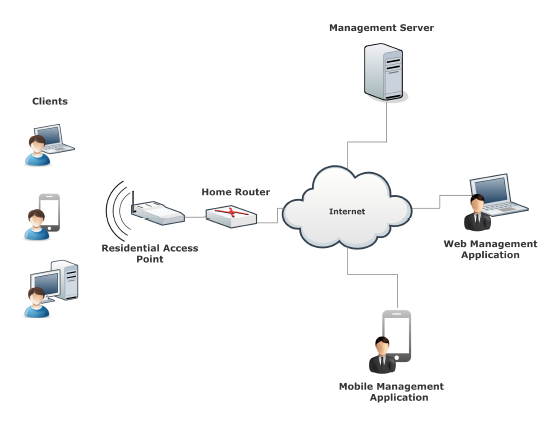
\includegraphics[width=0.80\textwidth,natwidth=610,natheight=642]{figs/presystem.png}
  	\caption{Existing System Architecture}
  	\label{fig:presystem}
\end{figure}

\section{Improvement of Existing System}
\par According to the master project report \cite{TorgeirMR}, there are several function requirements mentioned in that report. In this project, the improvement functions of the system are shown in the Table \ref{tab:improve_system_func}.
\begin{table}
\caption{\label{tab:improve_system_func}: Improvement Functions for System}
\centering
\begin{tabular}{| c | p{4cm} | p{6cm} | l |}
\hline
 No. & Title & Improvement Function & Importance \\ \hline
 1 & Block Internet Access & The residential access point can block clients internet access base on MAC and forbid the \gls{ip} address request & High \\
 2 & Bug Fixed for static \gls{ip} lease & Bug found in the report with wrong script format in static \gls{ip} lease for residential access point & High \\
 3 & Bug Fixed for Missing script & Bug found in the report without essential script file & High \\
 4 & Broken \gls{sd} card changed & Changed broken \gls{sd} card in the project & High \\ \hline
 5 & Security Log on service & Implement security log on mechanism for mobile log on request & High \\
 6 & Complete Authenticate Log on service & Complete implementation of authenticate log on by user-name and password & High \\
 7 & Separate working protocol & Separate client request protocol and mobile management application working protocol on central management server & Medium \\
 8 & Set up Database Management Tool & Set up phpmyadmin\cite{phpmyadmin} to manage database on the central management server & High \\
 9 & E-mail Notification Mechanism & Implement E-mail notification mechanism on central management server to notify the client user internet access request & High \\ \hline
 10 & Security Log on & Implement security log on function on both android and \gls{ios} mobile application & High \\
 11 & Approve and Block Internet access & \gls{ios} Mobile Application can approve and block the client internet access request & High \\
 12 & Real-time update & \gls{ios} Mobile Application can real-time update all the client internet access request & Medium \\ \hline
\end{tabular} 
\end{table}

\section{Analysis of System}
\par The system is based on client-server model \cite{csmodel}, which is a distributed application structure in computing that partitions tasks or workloads between the providers of a resource or service, called servers, and service requesters, called clients. Since in the internet access system, the request client users connect with the residential access point (in this project will be \gls{rpi}), so it is better for the service to provide client-server model communication between different client users and residential access point. 
\par Moreover, there will be different residential access point from different residential areas to communicate with the same service provider (central management server) since the central management server will provide the server back-end service and store the database with information for administrator authentication , different residential \gls{macaddress} address and other necessary service data. The main database of the system should be able to be managed and modified by the administrators. Then the client-server model also would suit into this scenario.
\par According to the communication between mobile application clients and central management server, the client-server model of this architecture is better for central management server to return the response of the \gls{http} request and manage the whole service of the system.
\par More detail about the different components in system architecture would be covered in the individual chapter \ref{chp:rpi}, chapter \ref{chp:central_server} and chapter \ref{chp:mobile_app}.
\par Because there is no running system from previous student master project when this project begin, the performance between previous system and current improvement system would not be compared in this report. However, different improvement of the internet access system would be discussed in the later chapters. And all improvement functions would be only based on the master project report\cite{TorgeirMR}.

\begin{figure}
	\centering
    	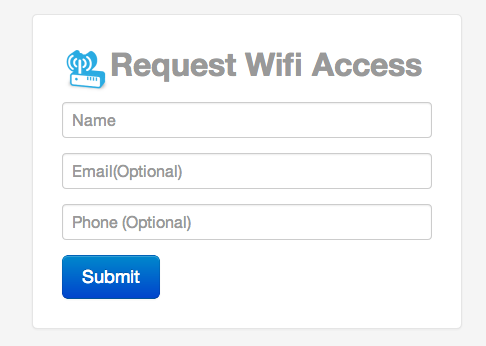
\includegraphics[width=0.60\textwidth,natwidth=610,natheight=642]{figs/wifi_request_page.png}
  	\caption{Request Client User Web Request Page}
  	\label{fig:wifi_request_page}
\end{figure}

\section{User Case}
\par Normal user case for this prototype system will be discussed in this section. There are two children in Adam's family. One is 19-year-old daughter Stella and the other is 15-year-old son Aslak. Usually Adam and his wife Eva live with their younger son, they are using the same wireless network based on internet access control system in their house. However, Aslak likes to play online game too much and sleep very late. Then everyday around 2200, Adam will use his WifiAccess Manager application on his iPhone to block his son's computer internet access to make sure Aslak could sleep at the acceptable time everyday. Some weekend, his daughter come back to their house to enjoy the weekend with them. Stella will make her computer and mobile phone connect with the wireless network, then she use the browser to type any domain name in the address bar, she will be redirected to the same central management server to request internet access like the Figure \ref{fig:wifi_request_page}. Then she just type her name for the current device to make request. After she made request, there will be a notification e-mail send to Adam's phone since his administrator user on the WifiAccess Manager application is registered with this e-mail address. Then Adam will use the ios application to approve this request, after that his daughter can connect with the internet this weekend.

\par More working process will be discussed in the Chapter \ref{chp:system_test}. There will be more detail system testing result in that Chapter.